% This file was created with tikzplotlib v0.10.1.
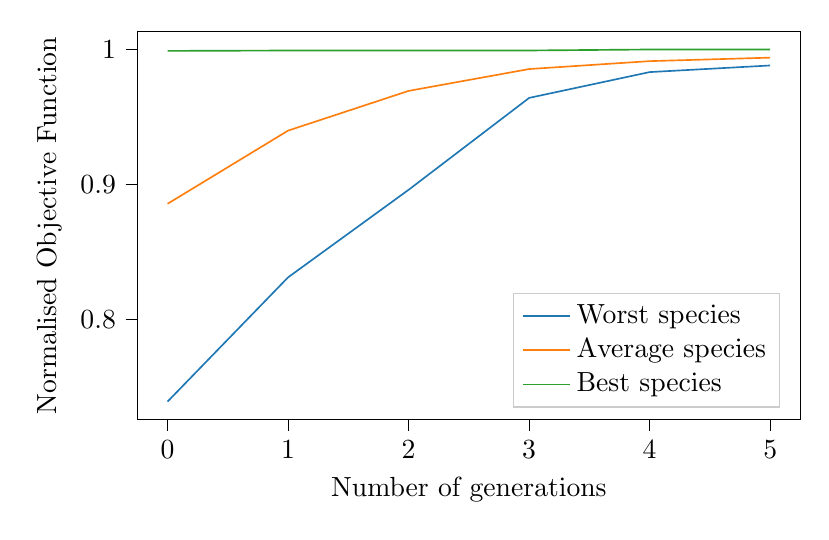
\begin{tikzpicture}

\definecolor{darkgray176}{RGB}{176,176,176}
\definecolor{darkorange25512714}{RGB}{255,127,14}
\definecolor{forestgreen4416044}{RGB}{44,160,44}
\definecolor{lightgray204}{RGB}{204,204,204}
\definecolor{steelblue31119180}{RGB}{31,119,180}

\begin{axis}[
legend cell align={left},
legend style={
  fill opacity=0.8,
  draw opacity=1,
  text opacity=1,
  at={(0.97,0.03)},
  anchor=south east,
  draw=lightgray204
},
tick align=outside,
tick pos=left,
x grid style={darkgray176},
xlabel={Number of generations},
xmin=-0.25, xmax=5.25,
xtick style={color=black},
y grid style={darkgray176},
ylabel={Normalised Objective Function},
ymin=0.726233588410974, ymax=1.01303649578995,
ytick style={color=black},
width=10cm, height=6.5cm
]
\addplot [semithick, steelblue31119180]
table {%
0 0.739270084200928
1 0.831286401892712
2 0.896101262018866
3 0.964155681818558
4 0.983271267438304
5 0.988170302509499
};
\addlegendentry{Worst species}
\addplot [semithick, darkorange25512714]
table {%
0 0.885742046673712
1 0.939937763667697
2 0.969348847053859
3 0.985528356188027
4 0.991381693941551
5 0.993972635888138
};
\addlegendentry{Average species}
\addplot [semithick, forestgreen4416044]
table {%
0 0.998964995578865
1 0.999244067375128
2 0.999273091868677
3 0.999273091868677
4 1
5 1
};
\addlegendentry{Best species}
\end{axis}

\end{tikzpicture}
